\section{Das IceCube-Experiment}
\label{sec:detector}
Der IceCube Detektor dient der Detektion von hochenergetischen  Neutrinos und Myonen und besteht aus drei Komponenten. Dem IceTop Detektor, dem In-Ice Detektor welche die gr\"o\ss te Komponente ist und dem DeepCore.
Das Experiment befindet aich am geographischen S\"udpol und die die Hauptdetektionsschicht ist zwischen $\SI{1450}{\meter} - \SI{2450}{\meter}$ in einer klaren Eisschicht.
Mit Hilfe von Cherenkov Licht, welches mit 5160 DOMs\footnote{digital optical modules} an 86 strings detektiert werden kann, lassen sich hochenergetische geladene Teilchen detektieren.
Ein schematischer Aufbau ist in Abbildung \ref{fig:cube} gegeben.

\begin{figure}
  \centering
  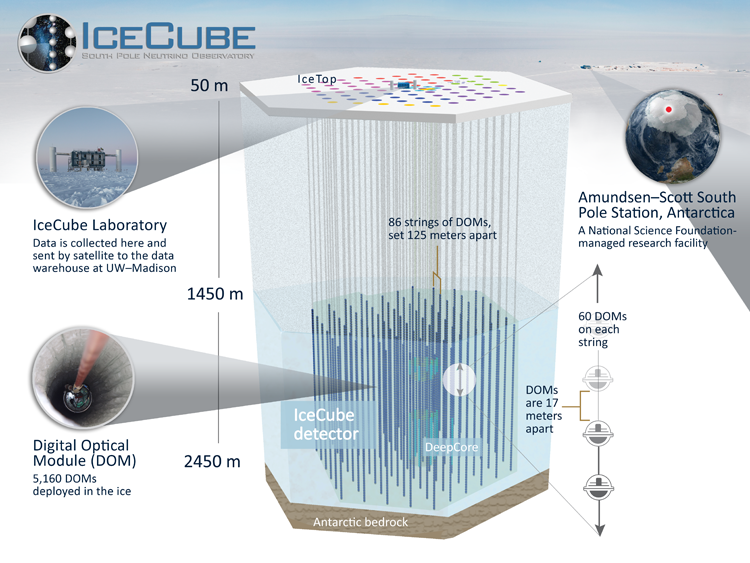
\includegraphics[width=0.8\textwidth]{plots/icecube_detector_sm.png}
  \caption{Schematischer Aufbau des IceCube Experiments.}
  \label{fig:cube}
\end{figure}

Das DeepCore besteht aus sieben Kabeln, welche sich im Zentrum des In-Ice Detektors befinden, l\"asst sich die Energieaufl\"osung dort auf $\SI{10}{\giga\electronvolt}$ senken gegen\"uber den $\SI{100}{\giga\electronvolt}$ des In-Ice Detektors.
Das IceTop dient als Luftschauer Experiment welches Cherenkov Licht in lichtdichten detektiert. Au\ss erdem kann es als Vetoregion f\"ur das In-Ice verwendet werden um gewisse Winkelbereiche auszuschlie\ss en.

Die Prozesse zur Detektion von Neutrinos geschieht \"uber Sekund\"arteilchen aus den Wechselwirkungen mit den Kernen im Eis als geladener Strom
\begin{equation*}
  \nu_l (\bar{\nu}_l) + A \to l^{\mp} + X
\end{equation*}
oder neutraler Strom
\begin{equation*}
  \nu_l + A \to \nu_l + X\,.
\end{equation*}

Hierbei verursachen Elektronen eine sph\"arischen Schauer aufgrund des rapiden Energieverlustes. Myonen hingegen haben einen eher langsamen Energieverlust und k\"onnen gr\"o\ss ere Distanzen \"uberwinden und haben eine lange "Lichtspur" als Signatur. Tau-Leptonen haben eine \"ahnliche Signatur wie Elektronen aufgrund ihrer geringen Lebensdauer.
Myonen erzeugen zu wenig Cherenkov Licht um detektiert zu werden aber sie generieren Photonen und $e^+ e^-$ Paare im Medium, welche selbst wieder schauern und weitere Elektron-Positron Paare erzeugen und von den PMT\footnote{Photomultipliern} aufgesammelt wird.
